\subsection*{Problema 13}
\textbf{Enunciado:} Calcular la integral:
\begin{align*}
\int \dfrac{x^4 - 2x^3 + 3x^2 - x + 3}{x^3 - 2x^2 + 3x} \, dx
\end{align*}

\textbf{Solución:} Dado que el grado del polinomio numerador ($4$) es mayor que el grado del denominador ($3$), realizamos la división algebraica. Dividiendo el numerador entre el denominador:
\begin{align*}
\dfrac{x^4 - 2x^3 + 3x^2 - x + 3}{x^3 - 2x^2 + 3x} &= x + \dfrac{-x + 3}{x^3 - 2x^2 + 3x}
\end{align*}

El denominador se puede factorizar como:
\begin{align*}
x^3 - 2x^2 + 3x &= x(x^2 - 2x + 3)
\end{align*}

Aplicamos fracciones parciales al residuo:
\begin{align*}
\dfrac{-x + 3}{x(x^2 - 2x + 3)} &= \dfrac{A}{x} + \dfrac{Bx + C}{x^2 - 2x + 3}
\end{align*}

Multiplicando por el denominador común:
\begin{align*}
-x + 3 &= A(x^2 - 2x + 3) \\
&\quad + (Bx + C)x
\end{align*}

Agrupando términos semejantes:
\begin{align*}
-x + 3 &= (A + B)x^2 \\
&\quad + (-2A + C)x + 3A
\end{align*}

Igualando coeficientes:
\begin{align*}
A + B &= 0 \\
-2A + C &= -1 \\
3A &= 3 \implies A = 1
\end{align*}

Sustituyendo $A = 1$:
\begin{align*}
1 + B = 0 &\implies B = -1 \\
-2(1) + C = -1 &\implies C = 1
\end{align*}

Sustituyendo las fracciones parciales obtenidas:
\begin{align*}
\dfrac{-x + 3}{x^3 - 2x^2 + 3x} &= \dfrac{1}{x} + \dfrac{-x + 1}{x^2 - 2x + 3}
\end{align*}

Reintegrando toda la expresión:
\begin{align*}
\int \left( x + \dfrac{1}{x} - \dfrac{x - 1}{x^2 - 2x + 3} \right) dx
\end{align*}

Para la última integral, completamos la derivada del denominador en el numerador:
\begin{align*}
\dfrac{x - 1}{x^2 - 2x + 3} &= \dfrac{1}{2}\dfrac{2x - 2}{x^2 - 2x + 3}
\end{align*}

Integrando cada término:
\begin{align*}
\int x \, dx &= \dfrac{x^2}{2} \\
\int \dfrac{1}{x} \, dx &= \ln|x| \\
\int \dfrac{x - 1}{x^2 - 2x + 3} \, dx &= \dfrac{1}{2}\ln|x^2 - 2x + 3|
\end{align*}

Finalmente, la solución general de la integral es:
\begin{align*}
F(x) &= \dfrac{x^2}{2} + \ln|x| \\
&\quad - \dfrac{1}{2}\ln|x^2 - 2x + 3| + C
\end{align*}

\begin{figure}[H]
	\centering
	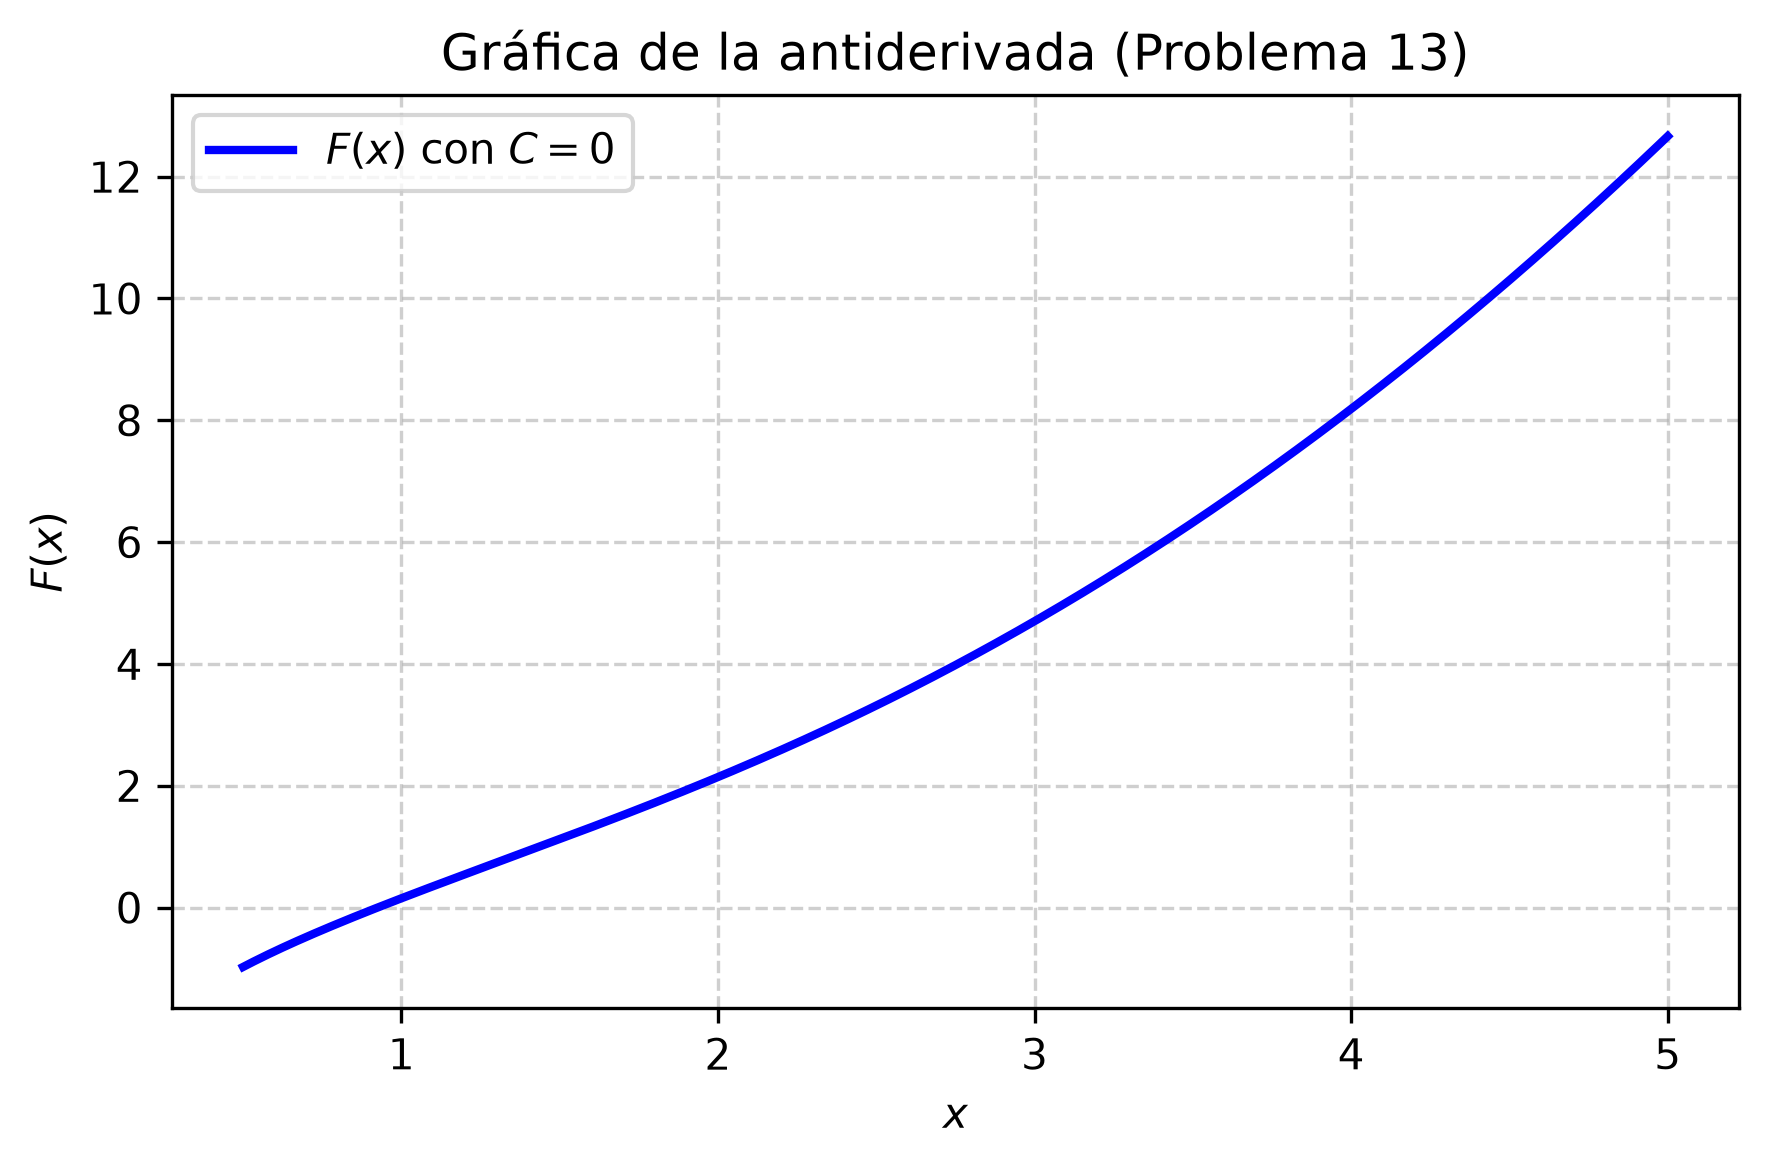
\includegraphics[width=\columnwidth]{semana_03/graficas/SEM03_P13_grafica.png}
	\caption{Representación gráfica de $f(x)$ y su antiderivada $F(x)$ evaluada para la constante de integración $C = 0$ (Problema 13).}
	\label{fig:problema13}
\end{figure}
